\section{Lí thuyết}
\begin{enumerate}
    \item Dụng cụ:
    \begin{itemize}
        \item Detector bán dẫn HPGe
        \item Nguồn neutron \ce{Am-Be}, cường độ 7Ci, thông lượng neutron nhiệt = $10^6 (n.cm^{-2}.s^{-1})$ 
        \item Mẫu so sánh: \ce{MnO2} , \ce{V2O5}, chứa chất nền graphit, tổng khối lượng $m_{hh} = 5 (g)$, là ống nhựa (đường kính 10mm, chiều cao 50mm).
        \item Mẫu phân tích: Tổng khối lượng $m_{hh} = 5 (g)$, có thành phần chứa nguyên tố quan tâm: \ce{Mn} và \ce{V}, trộn với chất nền acide Boric \ce{H3BO3}.
    \end{itemize}
    
    \item Phản ứng kích hoạt neutron:
        \begin{equation}
            \begin{cases}   
                ^{55}Mn (n,\gamma) ^{56}Mn\\
                ^{51}V (n,\gamma) ^{52}V
            \end{cases} 
        \end{equation}
     Cường độ phát gamma của đồng vị phóng xạ tỉ lệ với hàm lượng trong mẫu:
        \begin{equation}
            w = a + b.S 
        \end{equation}
    Trong đó: $w (g/g)$ là hàm lượng nguyên tố quan tâm, $S (counts)$ là diện tích đỉnh của đồng vị phóng xạ 
 
    \item Sai số dựa vào phương pháp bình phương tối thiểu:
    \begin{equation}
        \sigma_w = \sqrt{\sigma_a ^2 + S.\sigma_b^2}
    \end{equation}

    \item Đánh giá sai số của phương pháp đo.
      Theo như trong quá trình chuẩn bị mẫu, ta biết trước lượng \ce{MnO2} và \ce{V2O5} (trong bảng số liệu ~\ref{solieu}  và kết quả phân tích trong bảng ~\ref{phantich_w}  )
    \begin{align}
        \text{Sai số NAA (\%)} = \abs{\dfrac{w_{\text{Phan tich}}  - w_{\text{Li thuyet}} }{w_{\text{Li thuyet}}} .100 \%}
    \end{align}
\end{enumerate}

\section{Kết quả phân tích và nhận xét}
\begin{enumerate}
    \item Hàm lượng mẫu chuẩn của nguyên tố Mn trong \ce{MnO2}
    \begin{equation}
        w_i^* = \dfrac{m_i^*}{m_{hh}}.\dfrac{55}{87}
    \end{equation}
    \item Hàm lượng mẫu chuẩn của nguyên tố V trong \ce{V2O5}
    \begin{equation}
        w_i^* = \dfrac{m_i^*}{m_{hh}}.\dfrac{51*2}{182}
    \end{equation}

    \item Phương trình fit bình phương tối thiểu:\\
    Mn: $w_i =  (-0.008455 \pm 0.007353)  +  (  0.000185 \pm  0.000010 ) * S_i $\\
    Cr: $w_i = ( -0.012270 \pm   0.010212) +   (0.000735 \pm  0.000055 )* S_i $ 

    
\end{enumerate}


% Table generated by Excel2LaTeX from sheet 'Sheet1'
\begin{table}[htbp]
    \centering
    \caption{Bảng kết quả phân tích hàm lượng các nguyên tố Mn (Phản ứng  $^{55}Mn (n,\gamma) ^{56}Mn$  và nguyên tố V (Phản ứng $^{51}V (n,\gamma) ^{52}V$ - Units: Khối lượng mẫu m(g) ; Hàm lượng w (g/g), Diện tích đỉnh $S \pm \delta_S (\%)$ (counts)}
      \begin{tabular}{rllrrrrr}
    \hline
    STT     & Đồng vị & Tên mẫu & $E_\gamma (keV)$ & m(g) & Hàm lượng w & $S \pm \delta_S (\%)$ \\
    \hline
    0     & 56Mn  & SS1   & 846.8 & 0.5   & 0.063218 & $373 \pm 5.78$ \\
    1     & 56Mn  & SS2   & 846.8 & 0.8   & 0.101149 & $613  \pm 4.19$ \\
    2     & 56Mn  & SS3   & 846.8 & 1.5   & 0.189655 & $1062  \pm  3.15$ \\
    3     & 56Mn  & X1    & 846.8 & 1.2   & 0.160676 & $913   \pm  3.46$ \\
    4     & 56Mn  & X2    & 846.8 & 0.6   & 0.068052 & $413   \pm  5.29 $\\
    5     & 56Mn  & X3    & 846.8 & 0.6   & 0.075462 & $453   \pm  5.06 $\\\hline
    6     & 52V   & SS1   & 1434.1 & 1.5   & 0.168132 & $247   \pm  6.51$ \\
    7     & 52V   & SS2   & 1434.1 & 1.0   & 0.112088 & $164   \pm  8.09 $ \\
    8     & 52V   & SS3   & 1434.1 & 0.7   & 0.078462 & $127   \pm  9.67 $\\
    9     & 52V   & X1    & 1434.1 & 1.2   & 0.119315 & $179   \pm  8.41 $\\
    10    & 52V   & X2    & 1434.1 & 0.9   & 0.095792 & $147   \pm  9.19 $\\
    11    & 52V   & X3    & 1434.1 & 0.9   & 0.100937 & $154   \pm  8.66$ \\
    \hline
      \end{tabular}%
    \label{solieu}%
  \end{table}%
  


% Table generated by Excel2LaTeX from sheet 'Sheet1'
\begin{table}[htbp]
    \centering
    \caption{Bảng kết quả phân tích hàm lượng và đánh giá sai số; Units: Hàm lượng (g/g)}
      \begin{tabular}{rlrrrr}
    STT & Tên mẫu (Đồng vị) & w (Phân tích) & $\sigma_w$ & $w_{i}$ (Mẫu lí thuyết) & Sai số NAA (\%) \\
    \hline    
    0     & X1 - 56Mn  & 0.160676 & 0.007359 & 0.151724 & 5.900366 \\
    1     & X2 - 56Mn  & 0.068052 & 0.007356 & 0.075862 & 10.29444 \\
    2     & X3 - 56Mn  & 0.075462 & 0.007356 & 0.075862 & 0.526827 \\\hline
    3     & X1 - 52V   & 0.119315 & 0.010238 & 0.134505 & 11.29329 \\
    4     & X2 - 52V   & 0.095792 & 0.010233 & 0.100879 & 5.043105 \\
    5     & X3 - 52V   & 0.100937 & 0.010235 & 0.100879 & 0.057865 \\
    \hline
      \end{tabular}%
    \label{phantich_w}%
  \end{table}%
  
 
\begin{figure}
    \centering
    \begin{minipage}[htpb]{0.5\textwidth}
        \caption{Đường chuẩn w(mẫu chuẩn) Mn ($^{55}Mn (n,\gamma) ^{56}Mn$) - Units: w (g/g), Area(counts)}
        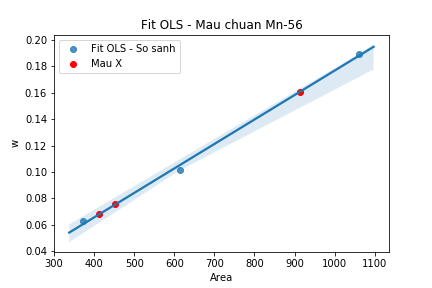
\includegraphics[width=\textwidth]{image/Mn.png}
    \end{minipage}
    \begin{minipage}[htpb]{0.5\textwidth}
        \caption{Đường chuẩn w(mẫu chuẩn) V ($^{51}V (n,\gamma) ^{52}V$) - Units: w (g/g), Area(counts)}
        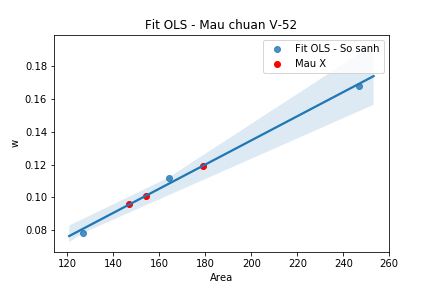
\includegraphics[width=\textwidth]{image/V.png}
    \end{minipage}
\end{figure}